\documentclass[10pt, a4paper, onecolumn, twoside, english]{article}
%MAY HAVE TO SPECIFY DOUBLE SIDED IF PRINTED IN THAT FORMAT
%unsure of any specific font size required
%"font size no smaller than 10pt"

\usepackage{everyshi}
\usepackage[absolute]{textpos}
%Phase One or phase one?
\usepackage{fullpage}
%at least 1 inch margins
\usepackage{amsmath}
%\usepackage{graphicx}
\usepackage{graphicx}

%\usepackage{lipsum}

%\renewcommand{\includegraphics}[2][]{%
%    \Huge$\times$% print x where image should be 
%}

\newcommand{\degree}{\ensuremath{^\circ}}

\usepackage{listings}
\usepackage{wrapfig}
\usepackage{color}
\usepackage{listings}
%special tabular environment
\usepackage{longtable}
%to set up page numbering
\usepackage{fancyhdr}
%to include the mission statement
\usepackage{pdfpages}
\usepackage{geometry}
%for inline whole citations:
\usepackage{bibentry}
\nobibliography*
% scientific notation, 1\e{9} will print as 1x10^9
\providecommand{\e}[1]{\ensuremath{\times 10^{#1}}}
\usepackage{amsmath} % needed for pmatrix
\usepackage{booktabs} % Fancy tables
%include python package for some sorted lists - not working yet
%\usepackage{python}
\usepackage{setspace}
%solves problem of urls in bibliography
\usepackage{url}
%to evaluate text only page count
\usepackage{comment}
%for special maths symbols
\usepackage{amssymb}
%compact maths font?
%\usepackage{mathptmx}
%compact lists
\usepackage{paralist}
%activate in case of way way too long
%\usepackage{savetrees}
%for checkmarks
\usepackage{amsfonts}
%for tables
\usepackage{pgfplotstable}
%config for long tables
% replicate column names on top of every page of a multi-page table:
\usepackage[T1]{fontenc}
\usepackage[latin9]{inputenc}
\usepackage{array}
\usepackage{babel}
\providecommand{\tabularnewline}{\\}

%\excludecomment{align}
%format the whole report with one half line spacing
\onehalfspacing

\lstset{ %
language=Python,                % choose the language of the code
basicstyle=\footnotesize,       % the size of the fonts that are used for the code
numbers=left,                   % where to put the line-numbers
numberstyle=\footnotesize,      % the size of the fonts that are used for the line-numbers
stepnumber=1,                   % the step between two line-numbers. If it is 1 each line will be numbered
numbersep=5pt,                  % how far the line-numbers are from the code
backgroundcolor=\color{white},  % choose the background color. You must add \usepackage{color}
showspaces=false,               % show spaces adding particular underscores
showstringspaces=false,         % underline spaces within strings
showtabs=false,                 % show tabs within strings adding particular underscores
frame=single,           % adds a frame around the code
tabsize=2,          % sets default tabsize to 2 spaces
captionpos=b,           % sets the caption-position to bottom
breaklines=true,        % sets automatic line breaking
breakatwhitespace=false,    % sets if automatic breaks should only happen at whitespace
escapeinside={\%*}{*)}          % if you want to add a comment within your code
}

% Notes on diagram and graph formatting:
% monochrome preferred, colour only to be used when it makes an important difference
% must have a clear explanatory caption: "sufficient to make their purpose understandable without reference to the main text"
% of course, must be referenced if not my own
% numbering should be sorted out by LaTeX regardless
% not formatting but interesting to not that it's important to seek permission before using any diagrams or figures from other works

\graphicspath{{./}, {../images/}}

%footer and header formatting
\fancypagestyle{plain}{%
\fancyhf{} %
\fancyhead[RO,RE]{\thepage}%
\renewcommand{\headrulewidth}{0pt}%
\renewcommand{\headheight}{20pt}%
\renewcommand{\footrulewidth}{0.2pt}
}

%Appendix formatting
\newcounter{alphasect}
\def\alphainsection{0}

\let\oldsection=\section
\def\section{%
  \ifnum\alphainsection=1%
    \addtocounter{alphasect}{1}
  \fi%
\oldsection}%

\renewcommand\thesection{%
  \ifnum\alphainsection=1% 
    \Alph{alphasect}%
  \else%
    \arabic{section}%
  \fi%
}%

\newenvironment{alphasection}{%
  \ifnum\alphainsection=1%
    \errhelp={Let other blocks end at the beginning of the next block.}
    \errmessage{Nested Alpha section not allowed}
  \fi%
  \setcounter{alphasect}{0}
  \def\alphainsection{1}
}{%
  \setcounter{alphasect}{0}
  \def\alphainsection{0}
}%

\widowpenalty=500

%\includeonly{Appendices}

\begin{document}
%   title page first - geometry to place title to do
%   must be carefully positioned to appear in the window of the blue sheet
%    \pagestyle{empty}
    \begin{titlepage}


\begin{textblock}{6.85}(4.72,4.18)
\begin{center}
{\doublespacing
{\bfseries
Gavin Gray
} \\
{\small s0805516 \\
{\bfseries \large \sffamily
An Audio Band Sigma-Delta Modulator with 103dB SNDR
} \\
}
}
\end{center}
\end{textblock}

\newpage
\thispagestyle{empty}
\mbox{}


\end{titlepage}

%empty page here?
    
    %set to number figures, tables and equations
    \numberwithin{equation}{section}
    \numberwithin{figure}{section}
    \numberwithin{table}{section}

%prior to main text
    \setcounter{page}{1}
    \pagenumbering{roman}
    \pagestyle{plain}

%   Mission Statement
    %\includepdf[pages={1,2}]{mission_statement.pdf}
    
%   Abstract - do at the end
%    \include{Abstract}

%   Declaration of originality - to do 
    %\include{dec_orig}

%   Statement of achievement - couple of paragraphs covering what you achieved during the project
    %\include{statement_achievement}

%   table of contents    
    \tableofcontents
%    \pagebreak

%   list of symbols - try and fill in as equations enter report, THEN REVIEW AFTER
    %\include{symbol_list}
    %probably not enough time for this

%   Glossary - see above, REVIEW AFTER - sortable lists possible in latex
%    \include{Glossary}

%   list of tables
%    \listoftables

%   list of figures
%    \listoffigures

%    \pagebreak

%   Main Text here
%   at the start of the main text
    \setcounter{page}{1}
    \pagenumbering{arabic}

%OBLIGATORY SPELL CHECK REMINDER - NEVER REMOVE THIS

%\section{Requirements(from assignment)}
%\begin{enumerate}
%   \item ``Quality and clarity of the report. Correctly annotated figures, legible graphs and plots. Structure and flow of material. Presence of index, glossary, abstract and appendices. Quality of English. References to books, papers and technology information.'' - most of these things should come about as I write this - look for easy opportunities to ref books, papers etc
%%   "Format of the report is the same as for MSc or MEng reports, see Section 7.5.8 in the handbook" - this are the same settings as used for MEng so this is done
%    \item ``A table comparing the amplifier specifications with the actual performance attained should be included. For every specification:
%    \begin{enumerate}
%        \item Worst case
%        \item Monte-carlo
%        \item Extracted
%    \end{enumerate}
%    Where specifications are NOT met, a discussion should be included of the reasons, impact on ADC performance and required remedial actions.''
%    \item ``Device sizing. 
%    \begin{enumerate}   
%        \item All equations used in choosing device sizes should be included. 
%        \item Where the actual device dimensions depart from those calculated, a discussion should be included.
%        \item Sizing of cascode bias generation circuits and choice of cascode voltages must be covered.''
%    \end{enumerate}
%    \item ``DC operating point. A table showing the dc operating point of the amplifier (in unity gain feedback) has been studied in the main process corners and that all devices are in saturation (apart from the common-mode feedback devices).'' - should make sure to also include the transistors in the CMFB amps.
%    \item ``{\bf Worst case} simulations of the amplifier specifications including plots of:
%    \begin{enumerate}
%        \item GBW
%        \item phase margin
%        \item PSRR
%        \item Settling
%        \item Common mode tracking
%        \item Output swing
%    \end{enumerate}
%    A discussion of any corners failing specifications must also be included.''
%    \item ``Plot of Monte-Carlo simulations of offset, PSRR, gain, GBW, phase, common mode tracking and output swing. A discussion of the effect of mismatch and actions taken to reduce the variation under Monte Carlo should be included'' - one of the only required pieces of explanation?
%    \item ``A plot showing a screen capture (colour) of your top-level layout overlaid with text showing the main sub-blocks. You should include a discussion of the overall layout strategy and floorplan. Any special steps to ensure noise immunity({\bf Shielding}) and matching({\bf common centroid}).''
%    \item ``Evidence of succesful verification of complete layout of amplifier. Print-out of LVS and DRC check results.'' - fairly easy, should explain the ERCs quickly.
%    \item ``Post-layout extracted simulations of all specifications. Discussion of departure of extracted amplifier performance from that of the schematic.'' - Extraction section should cover this, obviously.
%    \item ``ADC top-level simulations. Simulation of ADC at several input voltages with final MOS amplifier confirming correct code values. Comparison with macro-model performance. Check of worst case conditions on ADC accuracy.'' - This is still pending.
%    \item ``Added-value. Exploration of alternative circuit topologies, optimisation of power consumption, transistor-level implementation of other ADC blocks, sophisticated simulation techniques, demonstration of 10-bit ADC performance for all codes, corners and Monte-Carlo.'' - gain boosted design results (and problems), ENOB test using coherent sampling run over corners and Monte Carlo. Can then also state a FOM for the ADC, which would be nice.
%\end{enumerate}


%MAIN TEXT GOES HERE
%intro section
\section{Introduction}
%just a couple of paragraphs introducing the report
This report details the design a Sigma-Delta modulator in a design exercise.
The specifications of this modulator are described in section \ref{Design}.
Full simulation of the design in macro-model in Cadence was not completed due to time constraints but no problems are anticipated.

%
Time constraints were aggravated due to experimentation with a CIFB design that required extensive modification in Simulink to be succesfully verified.
Unfortunately, there were many bugs encountered due to inexperience editing Simulink models.
Finally, this design was abandoned in favour of a more established design that could meet the specifications.

A 2+1 MASH converter was chosen with an OSR of 128 to give adequate margin on the specifications.
It is shown that this is a robust design that is capable of meeting the specifications.
Due to time constraints it was not feasible to implement all the required extra blocks to build this modulator in Cadence.
Verification of the operation of the macro-model was performed on a first order modulator instead, as most noise is expected to be attributed to the first stage.


%subsections:
%   Specifications
%   Cyclic ADC Operation?

\section{Design}
\label{Design}
%section on all the design details
The required specifications are shown in table \ref{tab:SDspec}.
These specifications are a relatively low signal bandwidth and a very high SNDR that is characteristic of an audio band ADC.
In this section different options are evaluated and chosen from to meet these specifications.

\begin{table}
    \begin{center}
    \caption{A summary of the specifications required for this Sigma-Delta ADC.}
    \label{tab:SDspec}
    \begin{tabular}{l l} 
        \toprule
        Specification   &   Value  \\
        \midrule
        Supply Voltage ($V_{dd}$)               & $3.3 V$              \\
        Differential Input Voltage              & $1.8 V_{rms}$        \\
        Reference voltage $V_{refn}$            & $ 0 V$               \\
        Refererence voltage $V_{refp}$          & $0.9 \times V_{dd}$  \\
        Signal to Noise Ratio                   & $103 dB$             \\
        Total Harmonic Distortion at full-scale & $-85 dB$             \\
        NO audio band limit cycles or tones     & N/A                  \\
        A flat audio band noise profile         & N/A                  \\
        Exclusive voltage references            & N/A                  \\
        Clock Frequency                         & $12.288 MHz$         \\
        \end{tabular}
    \end{center}
\end{table}


\subsection{Noise in  Switched Capacitor Integrators}
\label{Design:noise}
%estimating the capacitor sizes for different OSRs
%use this to compare designs
For any size of modulator the noise will be dominated by the first integrator at the input\cite{Henderson2013}.
Shown in table \ref{tab:capsizes} are the required input capacitor sizings for different OSRs and for a presumed SNDR of 106dB for a small margin on the specifications.
Also shown in table \ref{tab:capsizes} are the required $g_{m}$s of the amplifiers in the first integrator for these capacitor sizes and settling errors required.

Quantisation noise is intended to be a very small part of the noise budget(\cite{Steensgaard2004}, p.437) - making the initial SNDR target 123dB.
The capacitor sizes are found by equating the expected quantisation noise for a 123dB SNDR with the expected kT/C noise on the capacitor:
%example calculation
\begin{align}
    \frac{m k T}{C OSR} = N_{q}^{2} = \frac{V_{inRMS}^{2}}{10^{\frac{SNDR}{10}}} = \frac{1.8^{2}}{10^{\frac{106}{10}}} = 8.14\e{-11} \\
    C = \frac{m k T}{OSR N_{q}^{2}} = \frac{4 \times 1.23\e{-23} \times 293}{OSR \times 8.14\e{-11}} 
\end{align}
%explain symbols here
Where $V_{inRMS}$ is the RMS differential voltage range and $m=4$ for a differential circuit.

%assume linear settling for the g_m
To find the required $g_{m}$, linear settling is assumed, and the settling time is dependent on OSR:
\begin{align}
    \tau_{settling} = \frac{256\times T_{clk}}{2\times OSR}
\end{align}
Where $\tau_{settling}$ is the settling time.
To settle to within $\sqrt{8.14\e{-11}} = 9.02\e{-6} V_{RMS}$ over the $1.8 V_{RMS}$ range of the circuit:
\begin{align}
    e^{\frac{-\tau_{settling} g_{m}}{C}} = \frac{9.02\e{-6}}{1.8} \\
    g_{m}  = - \frac{C \times \ln{\frac{9.02\e{-6}}{1.8}}}{\tau_{settling}}
\end{align}

\begin{table}
    \begin{center}
    \caption{A table summarising the required capacitor sizes and amplifier $g_{m}$s for different OSRs.}
    \label{tab:capsizes}
    \begin{tabular}{l l p{0.3\textwidth}} 
    \toprule
    OSR & Required Capacitor Size (F) & Required Amplifier $g_{m}$ (S) \\ 
    \midrule
    2   &  8.855\e{-11}  & 2.305\e{-4}  \\
    4   &  4.427\e{-11}  & 2.305\e{-4}  \\
    8   &  2.214\e{-11}  & 2.305\e{-4}  \\
    16  &  1.107\e{-11}  & 2.305\e{-4}  \\
    32  &  5.534\e{-12}  & 2.305\e{-4}  \\
    64  &  2.767\e{-12}  & 2.305\e{-4}  \\
    128 &  1.384\e{-12}  & 2.305\e{-4}  \\
    256 &  6.918\e{-13}  & 2.305\e{-4}  \\
    \end{tabular}
    \end{center}
\end{table}


Neglecting second order effects it appears that there is no downside to choosing a high OSR in the design of a Sigma-Delta modulator.
Effects such as slew rate and switch delays will affect these problems, however.
Without more complex simulation analysis it is difficult to quantify these other effects and it can only be said that these effects will exist.
Therefore, a high OSR is recommended for this design.

\subsection{Modulator Choice}
%based on the different combinations of bits, order and OSR that could meet the required specification
Shown in table \ref{tab:modoptions} are the major possible options that are projected based on graphs by Schreier \& Temes(\cite{Schreier2004}, p.112-113) and lecture notes.
This list is also limited to the options that are possible using the provided tools.

%list all the optimised cifb designs
%and MASH options
%and silva-steensgard
%and multiple bit quantiser designs
\begin{table}
    \begin{center}
    \caption{A table summarising design options evaluated during the design.}
    \label{tab:modoptions}
    \begin{tabular}{l l l p{0.2\textwidth} p{0.2\textwidth}}
    \toprule
    Architecture  & Order &   OSR     & Peak Nominal Observed SNDR(dB) & Notes \\
    \midrule
    CIFB & 3     & 128 & 109.0 & Margin on specifications not high enough. \\
    CIFB & 3     & 256 & 128.1 & \\
    MASH & 2+1   & 128 & 126.8 & Stable, established design. \\
    MASH & 1+1+1 & 128 & 126.9 & Error correcting abilities less effective than 2+1 design. \\
    %Silva-Steensgaard & 2 &  does not meet spec without multi-bit feedback
    %multi-bits go here
    \end{tabular}
    \end{center}
\end{table}


This list is reduced in that many of the CIFB designs are impossible to realise due to time constraints - they would require learning how to edit Simulink designs to add different quantisers and additional modulator stages.
Initial attempts to edit Simulink designs were unsuccessful, therefore limiting the possibilities to third order designs with different OSRs.

%discussion of MASH converter designs
It was possible to use MASH converter designs existing to meet the specifications with a lower OSR than would be required by a CIFB design.
Unfortunately it has been shown in section \ref{Design:noise} that this is not a first order concern - in fact, it is recommended to pick the highest possible OSR.
A problem with MASH converter designs anticipated would be noise leakage(\cite{Schreier2004}, p.132) - due to mismatches in the transfer functions of the different stages.

An additional problem with a MASH converter design is that simulations showed it would not have a completely flat audio band noise profile.
This can be seen in figure \ref{fig:MASHnominal} and can be compared with figure \ref{fig:cifbnominal}.

\begin{figure}
    \begin{center}
    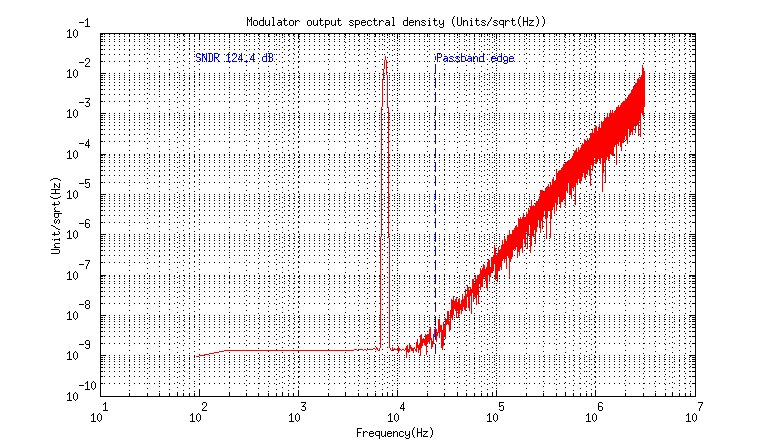
\includegraphics[width=0.8\textwidth]{MASHnominal.png}
    \caption{An example of a possible nominal MASH SNDR profile with a sine wave input.}
    \label{fig:MASHnominal}
    \end{center}
\end{figure}

\begin{figure}
    \begin{center}
    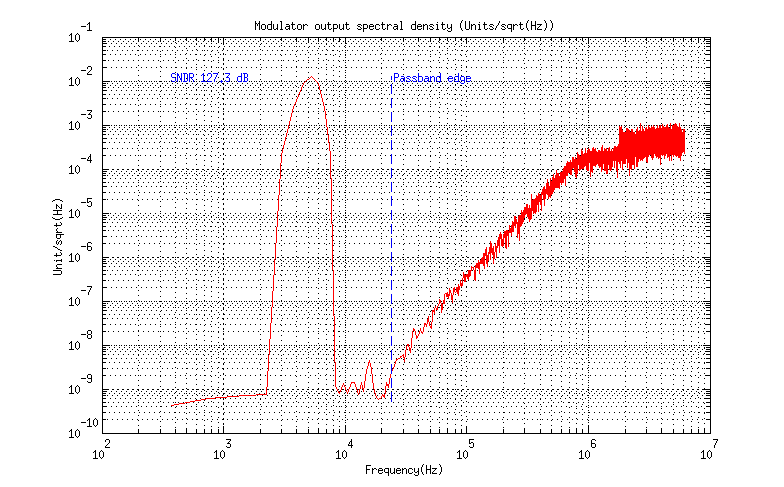
\includegraphics[width=0.8\textwidth]{cifbnominal.png}
    \caption{An example of a possible nominal CIFB SNDR profile with a sine wave input.}
    \label{fig:cifbnominal}
    \end{center}
\end{figure}

%need an argument against multi-bit feedback
%read textbook for this

%state choice and the reasons for the choice
Originally, a 3rd order CIFB design with an OSR of 256 was chosen as the design as it was able to meet the flat audio band noise profile requirement thanks to its optimised NTF.
Other advantages include it's simplicity with single-bit feedback and the anticipation of efficiency with the optimised transfer function.
Unfortunately, this design proved impossible due to stability and requirements for modification in Simulink that were unsuccessful.

The second choice was a MASH 2+1 converter with an OSR of 128.
Problems outlined above have been considered in the verification of the design in section \ref{Verification}.

    \subsection{Schematic}
    \label{Design:schematic}
    %top level diagram and some schematics showing how the sub-blocks should be implemented
    The top level functional diagram of a two stage 2+1 MASH modulator is shown in figure \ref{fig:MASH}.
    This design comprises several standard blocks that can be further broken down into their circuit implementations.

    %top level schematic
    %screencap from matlab
    \begin{figure}
        \begin{center}
        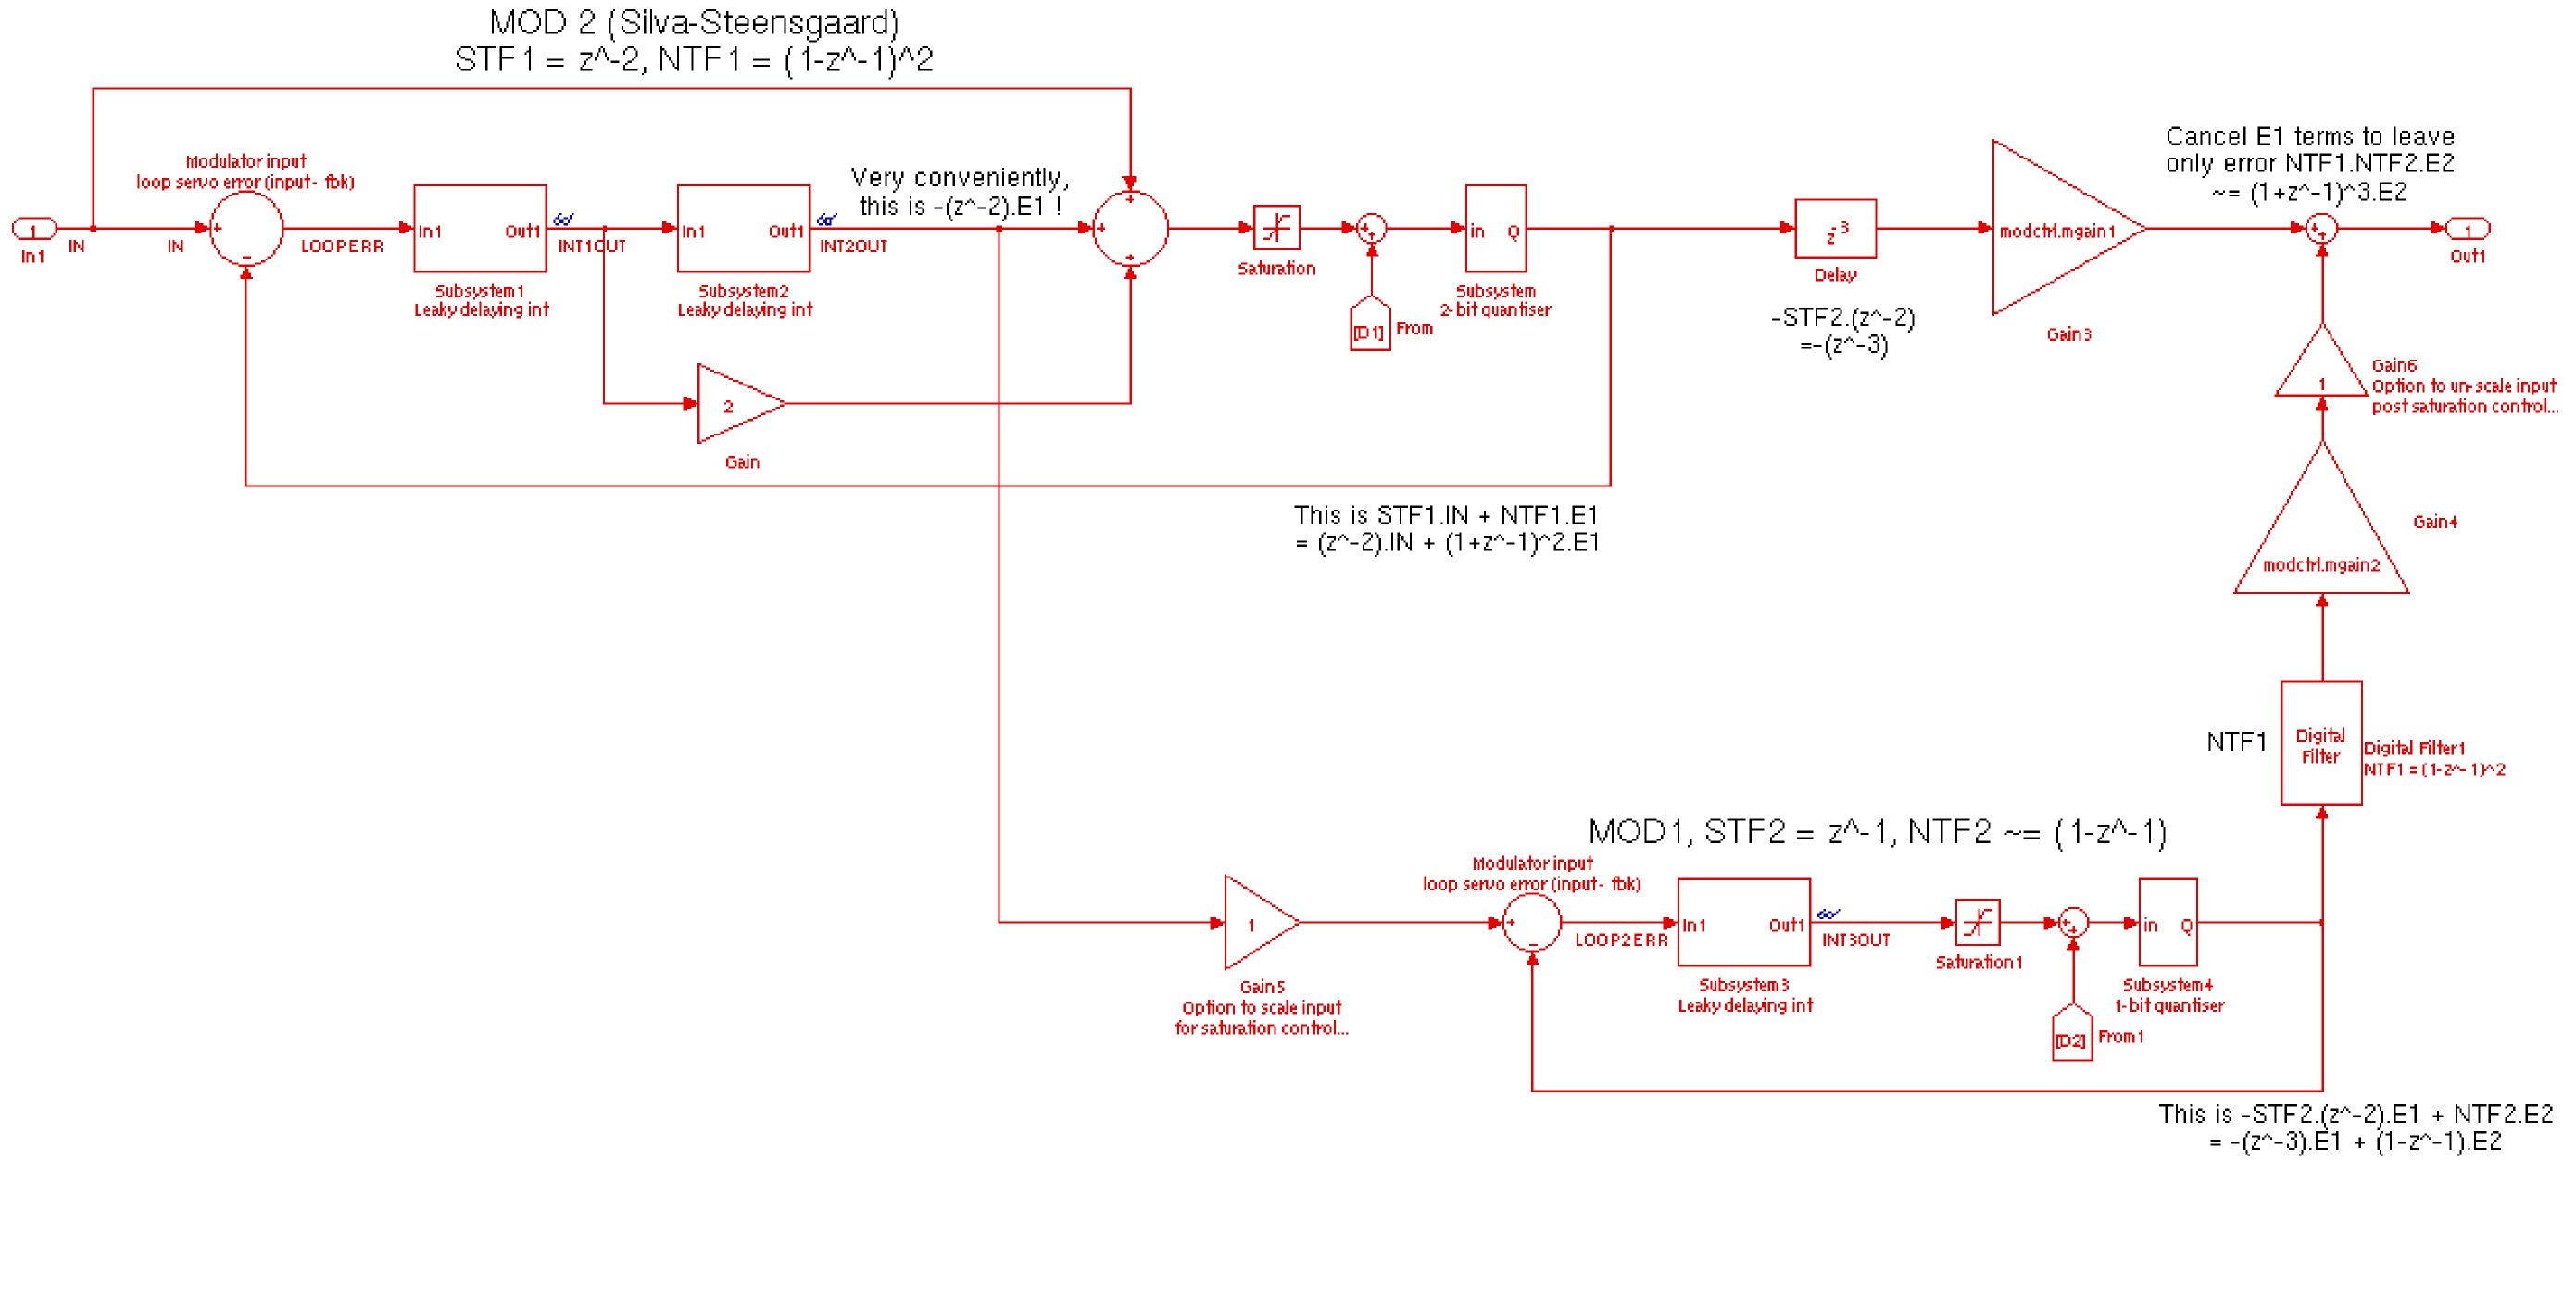
\includegraphics[width=0.8\textheight, angle=90]{MASH.png}
        \caption{Top level functional block diagram of the MASH modulator chosen in this design.}
        \label{fig:MASH}
        \end{center}
    \end{figure}

        \subsubsection{Silva-Steensgaard Modulator}
        %the second order modulator
        The first stage in this design is a second order modulator in a configuration known as a Silva-Steensgaard modulator.
        A differential circuit implementation of this circuit is shown in figure \ref{fig:silvaschematic}.

        \begin{figure}
            \begin{center}
            \includegraphics[width=0.8\textheight, angle=90]{silvaschematic.png}
            \caption{A differential implementation on the Silva-Steensgaard modulator.}
            \label{fig:silvaschematic}
            \end{center}
        \end{figure}

        %how to implement gain elements, coefficients, etc
        The gain elements and summing elements in this part of the design are implemented using capacitors.
        A differential multi-bit ADC and DAC must be implemented for this design to be created.
        A flash ADC implements the 2-bit ADC and an example circuit seen in figure \ref{fig:multiDAC} could be used to create the reference voltages if applied differentially.

        \begin{figure}
            \begin{center}
            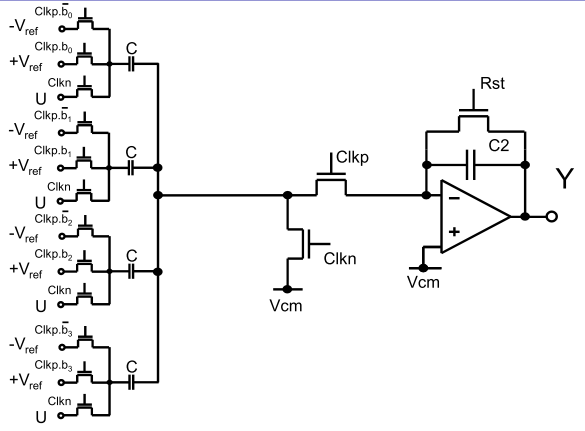
\includegraphics[width=0.8\textwidth]{multiDAC.png}
            \caption{A multi-bit DAC switched capacitor implementation\cite{Henderson2013a}.}
            \label{fig:multiDAC}
            \end{center}
        \end{figure}       

        %integrator design
        \subsubsection{First Order Modulator}
        %image and description of a differential integrator
        An example schematic for the first order modulator involved in this design is shown in figure \ref{fig:diffint}.
        This is the second modulator in the design and is a standard differential modulator design.

        %image should cite the lecture notes
        \begin{figure}
            \begin{center}
            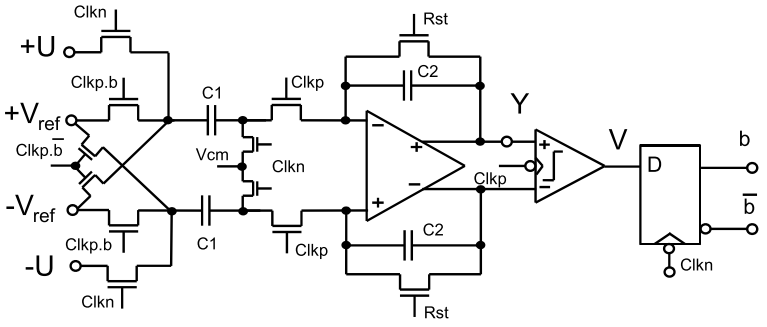
\includegraphics[width=0.8\textwidth]{diffint.png}
            \caption{A differential implementation of a first order modulator\cite{Henderson2013a}.}
            \label{fig:diffint}
            \end{center}
        \end{figure}

        %for the 1 bit quantiser
        A latched comparator is required to implement the single bit quantiser in the design.
        Designing this is a transistor level piece of design, and was not included in the design of the circuit.

        \subsubsection{Digital Signal Processing}
        %the filters, gain and digital summing elements
        The final signal processing in this modulator design is performed in the digital domain.
        A three cycle delay element, two gain operations and a summing element must be implemented in the digital design.
        This will also have to be combined with a digital filter after quantising prior to mixing.

        Without any of these components in the library available to the design at this point the implementation in Cadence could not be completed.
        It will be demonstrated that this design will be successful upon completion.

    \subsection{Component Sizing}
    \label{Design:components}
    %sizing of the capacitors and switches calculations
    The components in the first integrator are assumed to contribute the vast majority of the noise in the design.
    Due to this, only the switches and capacitors in this part of the design are considered in terms of their noise contribution.
    The required capacitor size for a 256 OSR and noise expectation comparable to an SQNR of 106dB is shown in table \ref{tab:capsizes}.

    The switches in the design must also be sized - similarly to the expected $g_{m}$ required for settling.
    Effective resistance of the switches must be designed in order that the voltage settles to within the required accuracy:   

    %take equation from above, then sub in R_on
    \begin{align}
        R_{switch}  = -\frac{\tau_{settling}}{C \ln{\frac{9.02\e{-6}}{1.8}}}
    \end{align}

    This evaluates to an effective switch resistance of $4819.59\Omega$.

    The required $g_{m}$ of the amplifier contributes to the required sizing of the input devices for the amplifier - along with estimations of bias currents required.
    An approximate minimum bias current can be estimated by the current required to slew the entire signal range in half a settling period.
    
    \begin{align}
        I = \frac{dV}{dt}C = \frac{2\times 1.8}{4.069\e{-8}}(6.918\e{-13}) = 6.121\e{-5} A
    \end{align}
    
    A bias current of approximately $100\mu A$ is therefore recommended in the input amplifier.
    Assuming an AMS process it is therefore possible to size the input devices for the settling requirements.
    
    \begin{align}
        g_{m} = \sqrt{\frac{2K'_{p} W |I_{D}|}{L}} \\
        \frac{W}{L} = \frac{g_{m}^{2}}{2K'_{p} |I_{D}|} = \frac{(2.305\e{-4})^{2}}{2(14\e{-6})(100\e{-6})} = 18.975
    \end{align}
    Where $K'_{p} = 14\mu A/V^{2}$ - assuming PMOS input devices for lower noise performance.
    Requirements for wider devices due to slewing or gain requirements could change this estimation, but it provides a lower bound.

    %remaining components, by estimating the noise factor of the amplifier
    The remaining components - switches and capacitors in the design - will all be sized smaller than those at the input as the input referred effect of these components will be negligible.
    Schreier \& Temes estimate the influence of capacitors in further stages to be approximately 0.01\%(\cite{Steensgaard2004}, p.441) of the input capacitor's contribution.
    From this, it can be estimated that capacitors of 20fF would be a safe value, and this would ease settling requirements in the circuit - switches could be up to 50 times more resistive, and therefore 50 times less wide.

\subsection{Conclusion}
\label{Design:conclusion}
%conclusion, write this at the end
The design of this circuit was mainly a process of choosing a modulator architecture and OSR.
Initial choices failed in simulation, forcing the choice of a dependable architecture.
A 2+1 MASH converter with an OSR of 128 was chosen and the sizes of the various components were estimated.


%subsections:

\section{Verification}
\label{Verification}
%section including all the simulation results created

    \subsection{DC Stability}
    \label{Verification:DCstab}
    %tests showing DC stability with different problems
    Tones at the output of a modulator will degrade the SQNR performance of a circuit during normal operation.
    Also, the effects of DC inputs on the stability of the loop must also be investigated to find the input range of the modulator over which it is stable. 
    The effect on output DC response from an input DC sweep due to finite amplifier gain is another important factor.
    The transient output of this modulator was inspected for various input voltages and found to be stable.

    %should have a plot of just the transient voltages at different points in the circuit for high input voltages to show nothing is becoming linear
    %GET RID OF THIS IF ITS DIFFICULT TO SOURCE THE WAVE
%    \begin{figure}
%        \begin{center}
%        \includegraphics[width=0.8\textwidth]{tranexample}
%        \label{fig:tranexample}
%        \caption{An example transient output waveform.}
%        \end{center}
%    \end{figure}


        \subsubsection{DC input voltage - DC output voltage}
        \label{Verification:DCinputoutput}
        %point out how this design's dead zone performance is better than for other designs
        %so it can be implemented using amplifiers with lower gain
        The effect of finite gain amplifiers on a design can be to cause ``dead zones'' to appear in the transfer function of DC input to DC output.
        This design is expected to be resistant to this effect as it is effectively a third order design and the width of the dead zone can be expected to be proportional to $\frac{1}{A^{3}}$.

        %there is no spec for this so could just drive it down very low
        The results of this design to this test are shown in figure \ref{fig:dcdc}.
        No dead zones are visible at any zoom level - the dead zones produced are smaller than the resolution of the sweep.
        This suggests it is likely the non-linearity will not affect the design.

        \begin{figure}
            \begin{center}
            \includegraphics[width=0.8\textwidth]{dcdc.png}
            \label{fig:dcdc}
            \caption{DC input voltage to DC output voltage for a finite gain of ...} %FILL IN THE GAIN HERE
            \end{center}
        \end{figure}       

        \subsection{DC input voltage - baseband power}
        \label{Verification:DCbbpwr}
        %
        A sweep of DC input voltages while monitoring the baseband power will detect tones appearing at those input voltages.
        The result of this test is shown in figure \ref{fig:dcdcbbpwr}.
        This was run with saturation limits in both integrators equal to 2.546V, to reflect the signal range required of the real circuits.

         \begin{figure}
            \begin{center}
            \includegraphics[width=0.8\textwidth]{dcdcbbpwrsweep.png}
            \label{fig:dcdcbbpwr}
            \caption{Nominal baseband power resulting from a sweep of DC inputs.}
            \end{center}
        \end{figure}       
        
        %this might result in requiring dither
        The baseband power never exceeds -103dB, so it can be expected that the circuit is well within specification.

        %investigate the effect of mismatch?

%    \subsection{Flat Noise Profile}
%    %using dither to make the noise profile flat
%    The noise profile of the chosen design without dither can be seen in figure \ref{fig:MASH}.
%    It does not meet the specifications in that it is not flat.
%    This is a problem that can be solved by applying dither to the circuit in the form of adding random noise at 
%
%    \begin{figure}
%        \begin{center}
%        \includegraphics[width=0.8\textwidth]{SQNRdither}
%        \label{fig:SQNRdither}
%        \caption{Single simulation showing the effect of dither on the noise floor of the modulator.}
%        \end{center}
%    \end{figure}  
%
%    Dither is therefore applied in all SQNR simulations involving this modulator.

    \subsection{SQNR Stability}
    %sweeps of SQNR
    To verify the performance of a Sigma-Delta modulator it's necessary to verify the resolution of the circuit at many input amplitudes and in cases involving non-ideal components.
    The cases tested here are:
    \begin{itemize}
        \item Capacitor mismatch
        \item Finite gain
        \item Stage mismatch
        \item Finite signal swing
    \end{itemize}

    Without mismatch, but with a finite gain of 1000 and a finite signal swing equal to that expected in the amplifier of 2.546V differential, the results of a sweep of input sine amplitudes is shown in figure \ref{fig:SQNRnominal}.

    \begin{figure}
        \begin{center}
        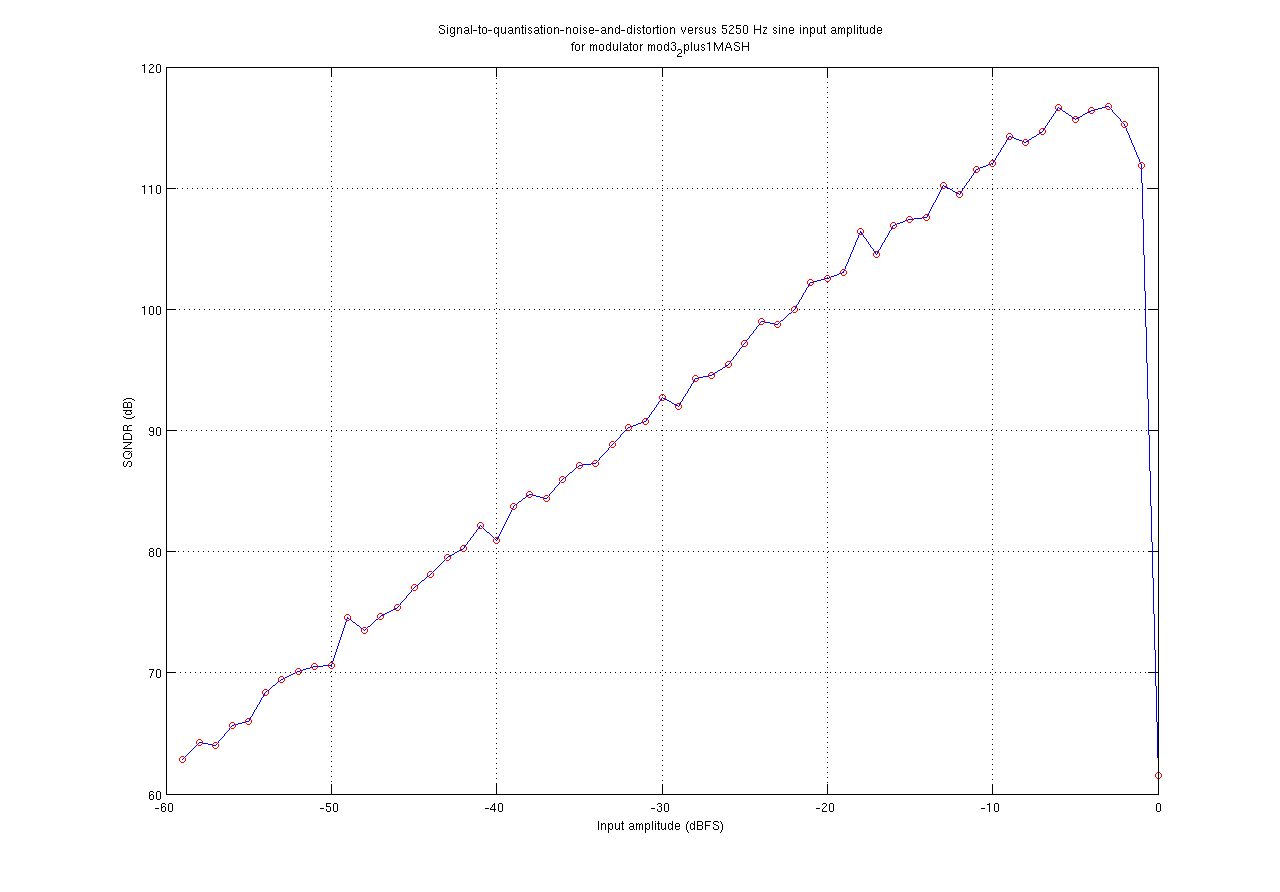
\includegraphics[width=0.8\textwidth]{MASHSQNRsweep0105.png}
        \label{fig:SQNRnominal}
        \caption{SQNR resulting from a sweep of different input amplitudes of a sine wave without mismatch is shown.}
        \end{center}
    \end{figure}  



        \subsubsection{Capacitor Mismatch}
        %capacitor mismatch, the effect of
        Capacitor mismatch causes a mismatch in the multiplication stages of the amplifier.
        In the matlab model there are various precise multiplication elements that can be varied.
        The variation expected in capacitors is 0.4\%, so a variation in these values of 0.4\% must be tested.
        For a design margin, this can be increased to 1\% mismatch on the two gains to modify in the design, shown in figure \ref{fig:MASH}.

        Applying gain mismatch of 1\% in all four possible configurations; the worst observed result is shown in figure \ref{fig:SQNRcap} - swept for all input amplitudes.
        The worst observed was a combination of 99\% mgain2 and 101\% mgain1.
        Figure \ref{fig:SQNRcap} shows that the circuit is still able to meet the specification.
 
        \begin{figure}
            \begin{center}
            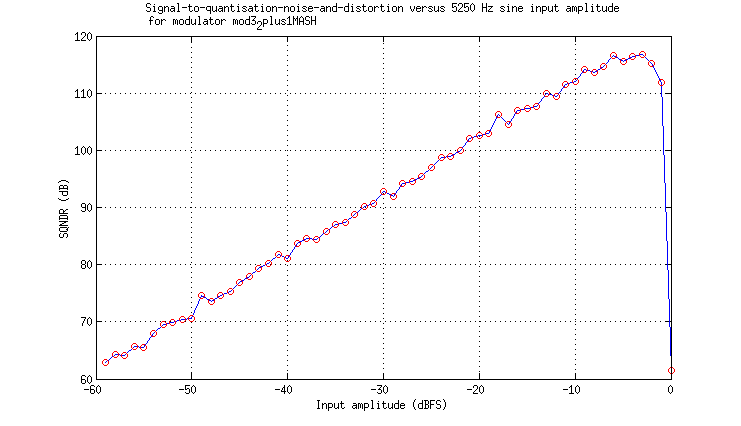
\includegraphics[width=0.8\textwidth]{MASHsweepcap.png}
            \label{fig:SQNRcap}
            \caption{SQNR resulting from a sweep of different input amplitudes of a sine wave with capacitor mismatch is shown.}
            \end{center}
        \end{figure} 

        \subsubsection{Effect of Noise Leakage} 
        %run SQNR sweeps with mismatches in the transfer function
        %reference equations describing this from the textbook
        Noise leakage is governed by the mismatch of transfer functions from the fist and second stages of the modulator(\cite{Schreier2004}, p.132).
        This requires modifying gain components defining the individual stages.
        With the worst case gains from the previous section set, these two internal gain blocks were modified by 1\% mismatch to find the worst combination.
        The result is shown in a sweep of all input amplitudes in figure \ref{fig:SQNRtrans}.

        \begin{figure}
            \begin{center}
            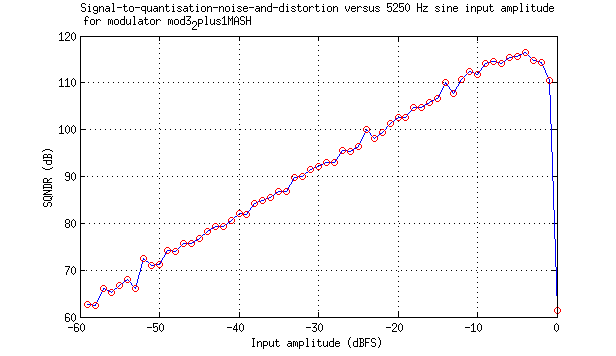
\includegraphics[width=0.8\textwidth]{MASHsweeptrans.png}
            \label{fig:SQNRtrans}
            \caption{SQNR resulting from a sweep of different input amplitudes of a sine wave with transfer function mismatch is shown.}
            \end{center}
        \end{figure} 

    \subsection{Cadence Tests}
    %test showing that the sizing of switches and caps is ok
    To show that the sizing of devices in section \ref{Design:components} is correct the modulator should be simulated to show that the input referred noise is as low as expected.
    Unfortunately, the full modulator was not implemented in Cadence, making this full simulation impossible.
    To prove that the sizing is adequate a first order modulator noise simulation was performed with the input capacitor and $g_{m}$ sizing calculated applied.

    %notes on resizing to meet specification
    First order calculations proved to be inaccurate at this point and it was necessary to further increase the size of the input capacitors to meet the noise requirements.


    %noise breakdown results showing the noise being within specification
    

    %estimate the SQNR that would be achieved by adding worst case quantisation noise and worst case thermal noise
   
 
    %make up a FOM?    


\subsection{Conclusion}
\label{Verification:conclusion}
%conclusion to the verification section
Although a full simulation of a macro-model implementation of the modulator has not been completed, the simulation results presented here show that this circuit is capable of meeting the specifications as described.
Non-ideal effects have been considered in the matlab simulations and noise has been investigated in the Cadence simulations.
From these results the circuit can be expected to work if completed.


%subsections:

\section{Conclusion}
\label{Conclusion}
This design exercise has resulted in a delta-sigma modulator design that is very likely to be successful.
It is expected that this modulator is able to meet the required SNDR specification.
Also, implementation and non-ideal component implications have been taken into account.



%
%           

%   References
    \bibliographystyle{vancouver}
    \bibliography{../../Bibtex/Sigma_Delta}{}

%  Appendices
%4.11.1. Additional material, e.g. mathematical derivations that may interrupt the flow of your paper's argument should form a separate Appendix section.
%Do not, however, use appendices to lengthen your article unnecessarily.
%If the material can be found in another work, cite this work rather than reproduce it. 
%4.11.2. Authors are encouraged to submit additional material as online supplementary material. This should be uploaded as an additional file during submission. 
    \begin{alphasection}
    \section{Appendices}

\subsection{Noise Results}
\label{Appendices:noise}
Below are the detailed noise results for the first order Sigma-Delta modulator simulated:

{\small
\begin{verbatim}
Device           Param    Noise Contribution    % Of Total
/MP1             fn       0.00109039            11.67     
/MP0             fn       0.00109039            11.67     
/MN5             fn       0.000967633           9.19      
/MN4             fn       0.000967632           9.19      
/MN2             id       0.000794298           6.19      
/MN3             id       0.000794297           6.19      
/MN5             id       0.000693841           4.72      
/MN4             id       0.000693841           4.72      
/MP1             id       0.000679872           4.54      
/MP0             id       0.000679869           4.54      
/ISAMP/MN0       id       0.000640003           4.02      
/ISAMN/MN0       id       0.000640003           4.02      
/MN3             rd       0.000524886           2.70      
/MN3             rs       0.000524886           2.70      
/MN2             rs       0.000524886           2.70      
/MN2             rd       0.000524885           2.70      
/MN1             id       0.000438385           1.89      
/MN0             id       0.000438382           1.89      
/ISAMP/MP0       id       0.000315646           0.98      
/ISAMN/MP0       id       0.000315646           0.98      
/IAMP/R0         rn       0.000310759           0.95      
/IAMP/R2         rn       0.000310757           0.95      
/MN2             fn       0.000143192           0.20      
/MN3             fn       0.000143175           0.20      
/MN0             fn       0.000134174           0.18      
/MN1             fn       0.000134169           0.18      
/ISAMP/MN0       fn       8.94553e-05           0.08      
/ISAMN/MN0       fn       8.94512e-05           0.08      
/ISAMN/MP0       fn       1.32172e-05           0.00      
/ISAMP/MP0       fn       1.32171e-05           0.00      
/MP1             rd       4.04961e-07           0.00      
/ISAMP/MP0       rd       3.85577e-07           0.00      
/MP0             rd       3.38168e-07           0.00      
/ISAMN/MP0       rd       3.38168e-07           0.00      
/MN4             rd       2.3952e-07            0.00      
/MN5             rd       2.39226e-07           0.00      
/MN1             rd       2.28542e-07           0.00      
/ISAMN/MN0       rd       2.21252e-07           0.00      
/MN0             rd       2.04225e-07           0.00      
/ISAMP/MN0       rd       2.04225e-07           0.00      
/I12/R1          rn       7.04327e-13           0.00      
/I12/R0          rn       2.57454e-14           0.00      
/MP1             rs       1.1224e-19            0.00      
/MN4             rs       8.2846e-20            0.00      
/MN5             rs       8.15679e-20           0.00      
/MN1             rs       6.73873e-20           0.00      
/ISAMN/MP0       rs       2.59885e-23           0.00      
/ISAMP/MP0       rs       2.06917e-23           0.00      
/MN0             rs       1.91568e-23           0.00      
/ISAMN/MN0       rs       1.09014e-23           0.00      
/ISAMP/MN0       rs       1.05909e-26           0.00      
/MP0             rs       1.84227e-27           0.00      
/IAMP/RODSINP    rn       0                     0.00      
/IAMP/RODSINP    fn       0                     0.00      
/IAMP/RNOISEP    rn       0                     0.00      
/IAMP/RNOISEP    fn       0                     0.00      
/IAMP/RNOISEN    rn       0                     0.00      
/IAMP/RNOISEN    fn       0                     0.00      
/IAMP/RDSINN     rn       0                     0.00      
/IAMP/RDSINN     fn       0                     0.00      
/IAMP/R2         fn       0                     0.00      
/IAMP/R0         fn       0                     0.00      
/I12/R1          fn       0                     0.00      
/I12/R0          fn       0                     0.00      

Integrated Noise Summary (in V) Sorted By Noise Contributors
Total Summarized Noise = 0.00319233
Total Input Referred Noise = 1.01957e-05
The above noise summary info is for pnoise data
\end{verbatim}
}


    \end{alphasection}

\end{document}
